% ---------------------------------------------------

\section{Sailboat Anatomy}
\label{app:sailboat_anatomy}

A sailboat consists of several key structural and functional components:

\begin{center}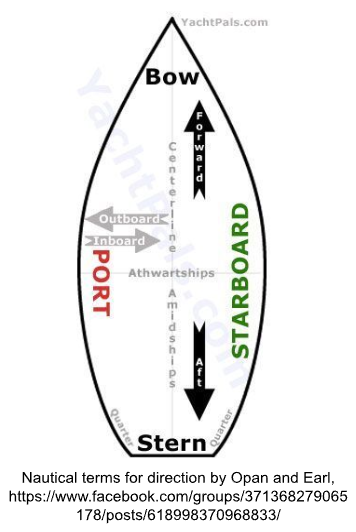
\includegraphics[width=0.6\columnwidth]{figures/images/boatAnatomy_directions.png}\end{center}

\textbf{Directions \& Regions:} Fore (forward) and aft (rearward) define movement along the longitudinal axis. Outboard (away from centerline) and inbaord (towards center line) refers to movement along the latitudinal axis. Bow is the front of the hull; stern is the rear. Starboard is the right side when facing forward; port is the left. 

\begin{center}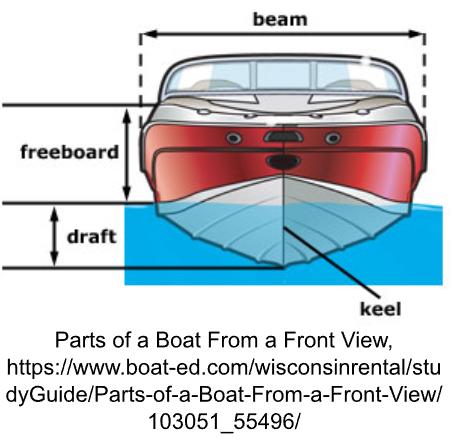
\includegraphics[width=0.6\columnwidth]{figures/images/boatAnatomy_waterLine.png}\end{center}

\textbf{Freeboard \& Draft:} Freeboard is the distance from the waterline to the deck. Draft is the distance from the waterline to the lowest point of the keel.

\begin{center}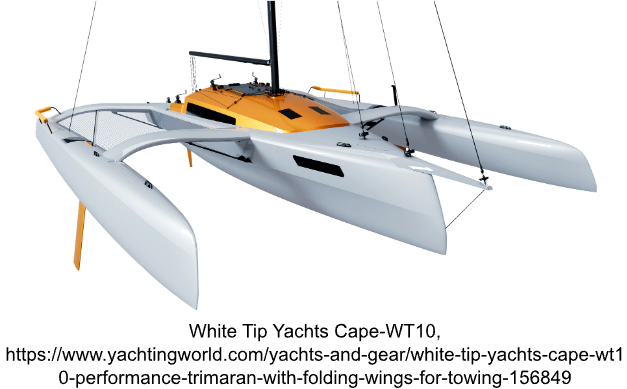
\includegraphics[width=0.6\columnwidth]{figures/images/Trimaran.png}\end{center}

\textbf{Hull:} The main body of the vessel providing buoyancy. Hull types include displacement hulls (slower, more stable) and planing hulls (faster, less stable). ALAN uses a trimaran configuration: a central vaka (main hull) with two amas (outriggers) connected by arms, providing exceptional stability.

\begin{center}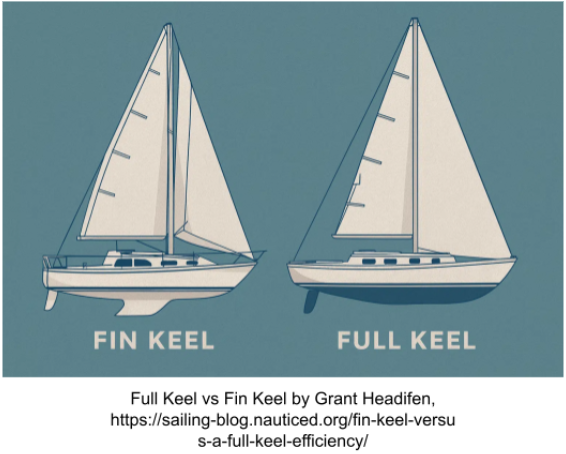
\includegraphics[width=0.6\columnwidth]{figures/images/boatAnatomy_keels.png}\end{center}

\textbf{Keel:} A fin extending below the hull that provides lateral resistance, preventing the boat from sliding sideways under sail force. Keel types include full keels (more stable, shallow draft, higher drag) and fin keels (more efficient, deeper draft). Sub-forms include squared, rounded, and bulb profiles. ALAN uses a fin keel with a bulb for stability and low center of mass.

\begin{center}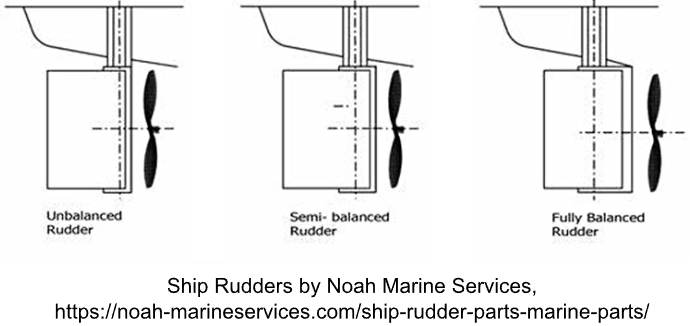
\includegraphics[width=0.6\columnwidth]{figures/images/boatAnatomy_rudders.png}\end{center}

\textbf{Rudder:} A movable fin at the stern used for steering. Balanced rudders are easy to turn but do not self-center; unbalanced rudders self-center but require more force. Styles include spade (free-floating, simple) and skeg-mounted (more protected, more stable). ALAN uses a spade rudder for simplicity.

\begin{center}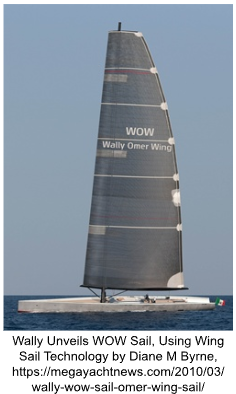
\includegraphics[width=0.6\columnwidth]{figures/images/boatAnatomy_wingSails.png}\end{center}

\textbf{Mast \& Sail:} The mast is a vertical bar supporting the sail. Sail materials include cloth (cheaper, traditional, more wear) and rigid (durable, more efficient lift). Autonomous boats favor rigid sails for durability.

\begin{center}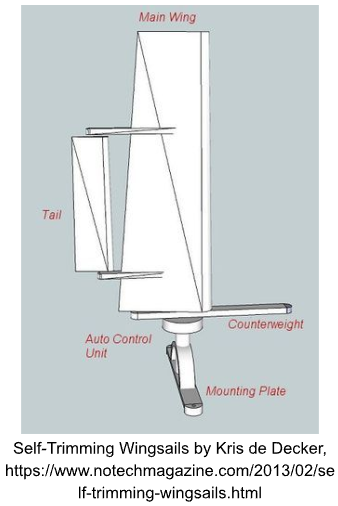
\includegraphics[width=0.6\columnwidth]{figures/images/selfTrimmingWingSail.png}\end{center}

\textbf{Self-Trimming Wingsail:} A rigid sail with a main element and a tail on a long rod aft of the pivot point. The tail provides passive aerodynamic torque to rotate the sail to the optimal angle. This design minimizes power consumption at the cost of higher mechanical complexity and wind-dependent response time.

% ---------------------------------------------------
